% !TeX root = ../main.tex

\section{Phonon}

\begin{problem}[Normal modes of a square lattice]
  Consider a square lattice of atoms of mass $M$,
  in which the nearest neighbors are coupled to each other
  by springs with constants $K$.
  Derive the equation of motion for the mode in which
  atomic displacements are normal to the crystal plane and
  find the dispersion of this mode.
  Analyze the behavior of this mode in the continuum limit.
\end{problem}
\begin{solution}[By TA]
  Only consider the vibration perpendicular to the surface
  \[
    M\odv[2]{U_{n,m}}t = -k \sum [u_{n,m} - u_{n\pm1,m\pm1}]
  \]
  Substitute the plane wave
  \[
    u_{n,m}(t) = U\upe^{\iu(q_xna + q_yna - \omega t)}
  \]
  we have
  \[
    -M\omega^2 = 2k[\cos(q_xa) + \cos(q_ya) - 2]
  \]
  For $|q_xa|$, $|q_ya| \ll q$, $\sin qa = qa$.
\end{solution}
\begin{solution}
  Assume the lattice constant $a$, then the lattice sites become
  \[
    \bm R_{n,m} = (na,ma), \quad n, m \in \mathbb Z.
  \]
  We consider every atom has a single degree of freedom: the out-of-plane scalar displacement $u_{n,m}(t)$. So, the spring connecting site $(n,m)$ and a neighbour $(n',m')$ has extension $\Delta = u_{n',m'} - u_{n,m}$, which brings the force to atom $(n,m)$
  \[
    F_{n,m} = -K(u_{n,m} - u_{n',m'})
  \]
  due to Hooke's law. Since every atom has four nearest neighbours:
  $(n \pm 1, m)$, $(n, m \pm 1)$, which bring four forces to the ``central atom''.
  Summing these forces
  \[
    F_{n,m}^\text{tot} = -\sum_{\braket<n,m;n',m'>} K(u_{n,m} - u_{n',m'})
  = -K(4u_{n,m} - u_{n+1,m} - u_{n-1,m} - u_{n,m+1} - u_{n,m-1})
  \]
  According to Newton's second law, we obtain the EOM
  \[
    M\ddot u_{n,m} = -K(4u_{n,m} - u_{n+1,m} - u_{n-1,m} - u_{n,m+1} - u_{n,m-1}).
  \]
  Assume the EOM has a plane-wave solution
  \[
    u_{n,m}(t) = A\upe^{\iu(k_xna+k_yma-\omega t)},
  \]
  then substitute it into the EOM, the LHS is
  \[
    \text{LHS} = M(-\omega^2)u_{n,m}
  \]
  and the RHS is
  \[
    \text{RHS} = -K(4 - \upe^{\iu k_xa} - \upe^{-\iu k_xa}
                      - \upe^{\iu k_ya} - \upe^{-\iu k_ya}) u_{n,m}
  = -2K[2 - \cos(k_xa) - \cos(k_ya)] u_{n,m}
  \]
  Finally we have the dispersion of this model
  \[
    \omega^2(\bm k) = \frac{2K}{M}[2 - \cos(k_xa) - \cos(k_ya)],\quad
    \omega(\bm k) = 2\sqrt{\frac KM} \sqrt{\sin^2\ab(\frac{k_xa}2) + \sin^2\ab(\frac{k_ya}2)}.
  \]
  In the continuum limit, i.e., $|\bm k|a \ll 1$,
  then the dispersion of this model becomes linear to $|\bm k|$
  \[
    \omega(\bm k) \approxeq
    2\sqrt{\frac KM} \sqrt{\ab(\frac{k_xa}2)^2 + \ab(\frac{k_ya}2)^2}
  = c|\bm k|
  \]
  where $c = a\sqrt{K/M}$.
\end{solution}

\clearpage

\begin{problem}[Localized phonons on an impurity]
  Consider a linear chain of identical atoms of mass $m$ each equidistant by $a$.
  \begin{enumext}[label = (\alph*)]
    \item Limiting the problem to interactions between nearest neighbors characterized by the force constant $\beta$, give the dispersion relation of longitudinal phonons and derive the expression of their group velocity.
    Express the results as a function of ``$a$'' and of the velocity of sound, $v_s$.
    What is maximum frequency of atomic vibration, $\omega_M$, when $v_s = \qty{5000}{\m/\s}$?
    \item An atom in the middle of the chain is replaced by the atom of an impurity with a mass $m'$ (where $m' < m$).
    Write the displacement equations, $u_0$, for this impurity atom and the displacement ``$u_n$'' for an atom located at a distance ``$na$''.
    Assume that the force constant $\beta$ between nearesst neighbors is the same regardless of the atom considered.
    \item The impurity atom being lighter than the others has an oscillation frequency $\omega_m'$ larger than $\omega_M$ and it drags the other neighbor atoms by its motion. We try to describe its effect with the expression of a damped wave of form: $u_n = u_0\upe^{-\alpha|x|} \upe^{\iu(\omega't-kx)}$.
    What is the value of the frequency $\omega_M'$, which is compatible with the equations of motion when the wave vector is near the boundary of the first Brillouin Zone? Verify that when $m = m'$, the solution matches that obtained in (a).
    \item After having numerically evaluated $\omega_M'$ and a when $m' = m/2$,
    sketch the instantaneous position of atoms as a function of $x$.
  \end{enumext}
\end{problem}
\begin{solution}[By TA]
  $v_y = \odv mk$.
  $v_s$ is long-wave limit $v_s$: $\lim_{k\to0}v_g = a\sqrt{\frac\beta m}$,
  and $\omega_m = \frac{2v_s}{a}$.
  \[
    u_n = u_0\upe^{-\alpha na}\upe^{\iu(\omega't - kna)}
  \]
  Substitute it into the EOM
  \[
    \begin{cases}
      -\omega'^2m' = \beta[\upe^{ax}(\upe^{\iu ka} + \upe^{-\iu ka}) - 2]\\
      -\omega'^2m = \beta[\upe^{(\alpha + \iu k)a} + \upe^{-(\alpha + \iu k)a} - 2]
    \end{cases}
  \]
  where $ka = \pi$, $\omega' = \omega_m'$,
  \[
    u_n = u_0(-1)^n \upe^{\iu\omega t} \upe^{-\alpha a|n|}
  \]
  \[
    \begin{cases}
      m\omega_m'^2 = 2\beta(1 + \upe^{-\alpha a}),\\
      m\omega'm^2 = \Delta\beta \cosh^2\ab(\frac{\alpha a}{2})
    \end{cases}
  \]
\end{solution}
\begin{solution}\leavevmode
  \begin{enumext}[label = (\alph*)]
    \item Assume the nearest-neighbor spring constant $\beta$.
    The EOM for the $n$-th atom is
    \[
      m\ddot u_n = -\beta(u_n - u_{n+1}) - \beta(u_n - u_{n-1})
    = \beta(u_{n+1} - u_{n-1} - 2u_n).
    \]
    We assume the EOM has a plane-wave solution
    $u_n(t) = A\upe^{\iu(kna-\omega t)}$, then substitute it into the EOM
    \[  
      -m\omega^2u_n = -\beta(2 - \upe^{\iu ka} - \upe^{-\iu ka})u_n
    = -\beta(2 - 2\cos(ka))u_n = -4\beta\sin^2\ab(\frac{ka}{2}),
    \]
    we have the dispersion
    \[
      \omega = 2\sqrt{\frac\beta m}\ab|\sin\ab(\frac{ka}{2})|.
    \]
    The group velocity and the velocity of sound are
    \[
      v_g(k) = \odv\omega k = a\sqrt{\frac\beta m} \cos\ab(\frac{ka}{2}),
      \qq{and}
      v_s(a) = \lim_{k\to0} v_g(k) = a\sqrt{\frac\beta m}
    \]
    then the group velocity, as well as the frequency can be expressed as
    \[
      v_g(k) = v_s \cos\ab(\frac{ka}{2}), \qq{and}
      \omega = \frac{2v_s}a \ab|\sin\ab(\frac{ka}{2})|.
    \]
    when $k = \pi/a$, the frequency arrives at a maximal value
    \[
      \omega_M = \frac{2v_s}{a} \xlongequal{v_s = \qty{5000}{\m/\s}}
      \frac{10000}{a} \unit{\s^{-1}}.
    \]
    \item The impurity is located at site $n = 0$, with mass $m'$;
    while its neighbors $n = \pm1$ with mass $m$.
    The EOM for the impurity and other atoms are
    \begin{align*}
      m'\ddot u_0 & = -\beta(u_1 - u_0) + \beta(u_{-1} - u_0)
    = \beta(u_1 + u_{-1} - 2u_0)\\
      m\ddot u_n & = \beta(u_{n+1} + u_{n-1} - 2u_n)
    \end{align*}
    \item In (a), near the boundary of the first BZ, i.e. $k = \pi/a$,
    the frequency is $\omega_\text I = 2\sqrt{\beta/m}$.
    Write the given wave form in terms of site number $n$
    \[
      u_n = A \upe^{-\alpha|n|a} \upe^{\iu(\omega't - kna)}
    \]
    Substitute it into the two EOMs in (b), and let $n = 1$
    \begin{align*}
      -\omega^2m'u_0 & = \beta(\upe^{-\alpha a-\iu ka} + \upe^{-\alpha a+\iu ka} - 2)u_0 \xlongequal{k = \pi/a} -2\beta(\upe^{-\alpha a} + 1) u_0\\
      -\omega^2m u_1 & = \beta(u_2 + u_0 - 2u_1) = \beta(\upe^{-\alpha a-\iu ka} + \upe^{\alpha a+\iu ka} - 2)u_1 \xlongequal{k = \pi/a}
      -2\beta(\cosh(\alpha a) + 1) u_1
    \end{align*}
    Derive the two expressions, we have
    \[
      \frac{m'}{m} = \frac{\upe^{-\alpha a} + 1}{\cosh(\alpha a) + 1}
    = \frac2{\upe^{\alpha a} + 1},
    \qq{and}
    \upe^{-\alpha a} + 1 = \frac{2m}{2m - m'}
    \]
    Substitute it into one of the EOM, we obtain the dispersion
    \[
      \omega_M'^2 = \omega'^2 = \frac{4\beta m}{m'(2m - m')}
    \]
    where $\omega_M'^2 = \omega'^2$ is due to the boundary of the first BZ ($k = \pi/a$).
    When $m' = m$, the frequency becomes
    \[
      \omega_M'^2 = \frac{4\beta}{m}, \qq{and} \omega_M' = 2\sqrt{\frac\beta m}
    = \omega_\text I
    \]
    which matchs that obtained in (a).
    \item Substitute $m' = m/2$ in the result of (c), we have
    $\omega_M'^2 = \frac{16}{3}\frac\beta m$.
    To simplify, we choose the time $t = 0$. Near the first BZ,
    the displacement of atoms is
    \[
      u_n = (-1)^n A\upe^{-\alpha|n|a}
    \]
    The plotted figure of atoms is attached as follows (Just show the relative position for reference).
    \begin{center}
      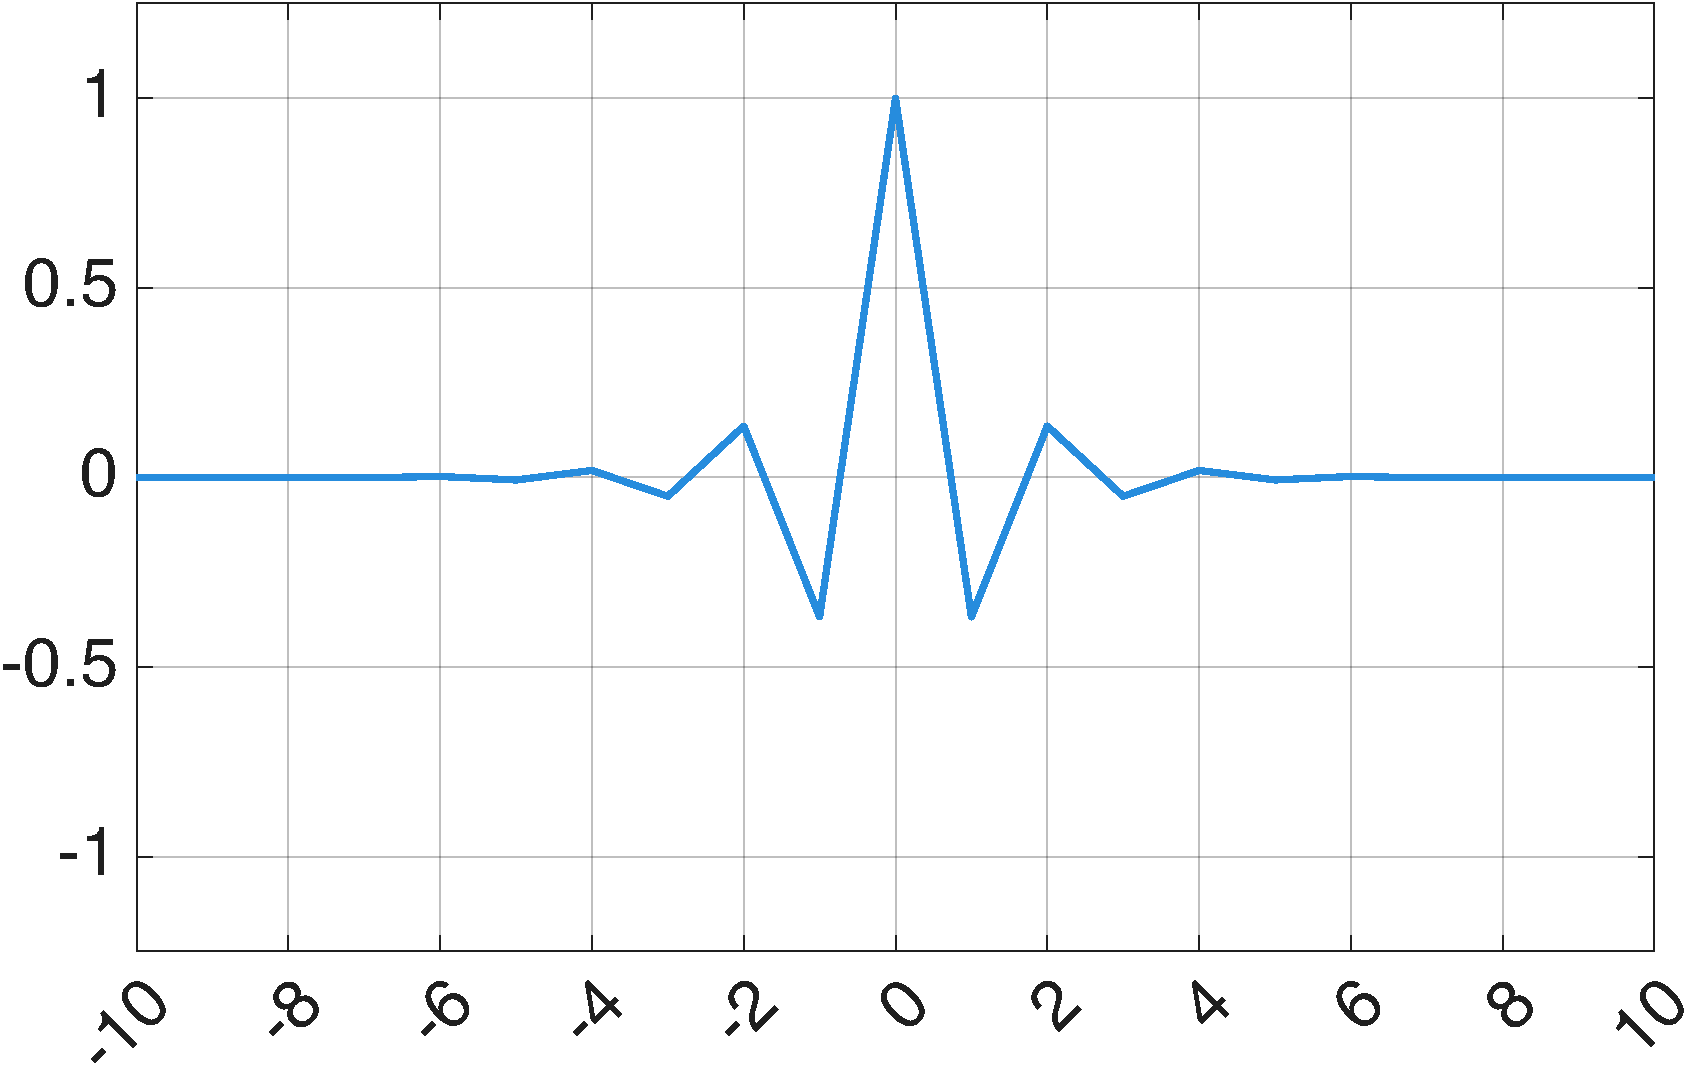
\includegraphics[width = .5\linewidth]{./media/hw2_fig.pdf}
    \end{center}
  \end{enumext}
\end{solution}

\clearpage

\begin{problem}[Density of states and specific heat of a monoatomic 1D lattice]
  Consider a row of $N$ identical atoms of mass $m$ and equidistant by $a$.
  \begin{enumext}[label = (\alph*)]
    \item Limiting the problem to interactions between nearest neighbors with a force constant $\beta$, find the expression for the dispersion relation of acoustic longitudinal vibrations propagating along this row. What is the maximum frequency $\omega_M$ of atomic vibrations, written in terms of $v_s$ and $a$? Compare the value obtained with that of $\omega_D$ deduced from the Debye model.
    \item Find the corresponding expression for the density of states $g(\omega)$.
    \item Write the expressions for internal energy $U$ and for the heat capacity $C_v$. Find the limits as these functions approach high temperatures ($\hbar\omega_M \ll k_BT$).
    \item What is the evolution of $C_v$ at low temperature? Compare the result obtained here with that deduced from the Debye model.
  \end{enumext}
\end{problem}
\begin{solution}[By TA]
  \begin{enumext}
    \item $\omega = v_sk$, $\int_0^{\omega_0} g_D(\omega) \d\omega = N$,
    $\omega(k) = 2\sqrt{\beta/m}|\sin(ka/2)|$.
    \[
      g_D(\omega) = \frac{L}{\pi} \odv k\omega = \frac L\pi \cdot \frac1{v_s}
    = \frac{Na}{\pi v_s}
    \]
    $\omega_D = \pi v_s/a$, $\omega_M = 2v_s/a$.
    \item $\braket<n> = \frac{1}{\upe^{\hbar\omega/k_BT} - 1}$,
    $\braket<E> = \braket<n>\hbar\omega$, $u_0 = \frac12\hbar\omega$.
    \[
      U = \int_0^{\omega_M} g(\omega) \ab[\frac12\hbar\omega + \frac{\hbar\omega}{\upe^{\hbar\omega/k_BT} - 1}] \d\omega
    \]
    $D_v = \odv UT$, for $\hbar\omega \ll k_BT$,
    the exponential is $\frac{\hbar\omega}{k_BT}$,
    \[
      C_v = k_B\int_0^{\omega_a} g(\omega) \d\omega = Nk_B
    \]
    \item Only $\omega \to 0$ contributes to the integration.
    \[
      \upe^{\hbar\omega/k_BT}
      \begin{cases}
        \hbar\omega \gg k_BT\frac{\hbar\omega}{\upe^{\hbar\omega k_BT}-1}
      = \hbar\omega\upe^{-\hbar\omega/k_BT},\\
        \hbar\omega \ll k_BT \upe^{\hbar\omega/k_BT} \approx k_BT
      \end{cases}
    \]
    $\omega \to 0$, $g(\omega) = g(0) = \frac{2N}{\pi\omega_M}$.
  \end{enumext}
\end{solution}
\begin{solution}\leavevmode
  \begin{enumext}[label = (\alph*)]
    \item The same to Problem 2.2(a): the dispersion
    \[
      \omega(k) = 2\sqrt{\frac\beta m}\ab|\sin\ab(\frac{ka}{2})|, ~
      v_s = \lim_{k\to0}\odv\omega k = a\sqrt{\frac\beta m}, \qq{and}
      \omega_M \xlongequal{k=\pi/a} 2\sqrt{\frac\beta m} = \frac{2v_s}{a},
    \]
    and the Debye frequency for 1D chain is $\omega_D = v_s k = \frac{\pi v_s}{a}$.
    Since $\omega_M/\omega_D = 2/\pi < 1$,
    the maximum frequency in the real dispersion is smaller than in the Debye model.
    \item In 1D chain, the number of states within $\d k$ is $2 \cdot \frac{L}{2\pi} \d k$. So, the density of states is
    \[
      g(\omega) = \frac L\pi \odv k\omega
    = \frac{2L}{\pi a\omega_M} \frac1{\sqrt{1 - (\omega/\omega_M)^2}}
    \xlongequal{L = Na} \frac{2N}{\pi\omega_M}
    \frac1{\sqrt{1 - (\omega/\omega_M)^2}}.
    \]
    \item The phonon thermal occupation
    \[
      n(\omega) = \ab[\exp\ab(\frac{\hbar\omega}{k_BT}) - 1]^{-1}
    \]
    Then the internal energy is
    \[
      U(T) = \int_0^{\omega_M} \hbar n(\omega) g(\omega) \d\omega
    = \int_0^{\omega_M} \frac{\hbar\omega}{\upe^{\frac{\hbar\omega}{k_BT}} - 1} g(\omega) \d\omega.
    \]
    and the heat capacity
    \[
      C_V(T) = \odv UT = \int_0^{\omega_M} \pdv{n(\omega)}T g(\omega) \d\omega
    \]
    At high-temperature limit, i.e., $\hbar\omega_M \ll k_BT$. The expression of internal energy and heat capacity become
    \[
      U(T) = \int_0^{\omega_M} k_BT g(\omega) \d\omega = Nk_BT,~
      C_V(T) = Nk_B.
    \]
    where applied the total number of vibration modes
    $\int_0^{\omega_M} g(\omega) \d\omega = N$.
    \newpage
    \item At low temperature limit, only small $k$ matters, i.e., the main contributions come from small $\omega$. Then, $g(\omega) = \frac L{\pi v_s}$.
    The internal energy becomes
    \[
      U = \frac L{\pi v_s} \int_0^\infty \frac{\hbar\omega}{\upe^{\frac{\hbar\omega}{k_BT}} - 1} \d\omega = \frac{\pi L(k_BT)^2}{6\hbar v_s}
    \]
    and the capacity
    \[
      C_v = \odv UT = \frac{\pi Nak_B^2T}{3\hbar v_s} \propto T
    \]
    the same conclusion as the Debye model.
  \end{enumext}
\end{solution}